\documentclass[11pt]{beamer}
\usetheme{Madrid}
\usefonttheme{serif}

\usepackage[utf8]{inputenc}
\usepackage[brazil]{babel}
\usepackage[T1]{fontenc}

\usepackage{amsmath}
\usepackage{amsfonts}
\usepackage{amssymb}
\usepackage{graphicx}

% Cores customizadas para dar um ar mais premium e alinhado com a UEA
\definecolor{ueablue}{RGB}{0,80,150}
\setbeamercolor{structure}{fg=ueablue}

\setbeamertemplate{caption}[numbered]

\title[Diálogos Dinâmicos em NPCs]{Avaliação de Modelos de Linguagem de Grande Escala na Geração Dinâmica de Diálogos para NPCs em Jogos de Investigação}
\author[João Lucas]{João Lucas Noronha de Castro \\ \small Orientador: Prof. Dr. Luis Cuevas Rodriguez}
\institute[UEA]{Universidade do Estado do Amazonas (UEA) \\ Curso de Sistemas de Informação}
\newcommand{\email}{jlnd.snf23@uea.edu.br}
\date{Junho de 2026}

% Comentado para fácil inclusão futura de logomarcas
% \logo{\includegraphics[scale=0.08]{imagens/logo_uea.png}}

\setbeamertemplate{navigation symbols}{}

\bibliographystyle{sbc} % Estilo SBC - arquivo sbc.bst copiado para a pasta slides

\begin{document}

\begin{frame}
\titlepage
\end{frame}

\begin{frame}{Sumário}
\tableofcontents
\end{frame}

\section{Introdução}

\begin{frame}{Introdução e Contextualização}
\begin{itemize}
    \item \textbf{Crescimento da Indústria:} Expansão do mercado de jogos digitais impulsiona a demanda por mundos virtuais mais ricos, imersivos e narrativamente complexos.
    \item \textbf{Narrativas de Alto Orçamento:} Ciclos de produção mais longos, equipes gigantescas e altos custos de desenvolvimento.
    \item \textbf{Inteligência Artificial Generativa:} Surge como alternativa para automatizar e escalar o design narrativo dinâmico de forma viável.
\end{itemize}
\end{frame}

\begin{frame}{O Problema: Árvores de Diálogo Estáticas}
\begin{columns}
\begin{column}{0.55\textwidth}
    \begin{itemize}
        \item \textbf{Rigidez Estrutural:} Diálogos tradicionais são sustentados por árvores determinísticas e pré-escritas \cite{ref1}.
        \item \textbf{Gargalo de Autoria:} Exige esforço manual exaustivo para criar todas as ramificações possíveis.
    \end{itemize}
\end{column}
\begin{column}{0.45\textwidth}
    \begin{figure}[htb]
        \centering
        
\includegraphics[width=\textwidth]{imagens/dialogue.jpg}
        \caption{\small Exemplo de diálogo em jogos.}
    \end{figure}
\end{column}
\end{columns}
\end{frame}

\begin{frame}{O Problema: Complexidade e Agência}
\begin{columns}
\begin{column}{0.55\textwidth}
    \begin{itemize}
        \item \textbf{Explosão Combinatória:} Rastrear múltiplos caminhos torna-se extremamente difícil e custoso para a equipe.
        \item \textbf{Limitação de Agência:} O jogador fica travado em opções pré-selecionadas de conversa, reduzindo a naturalidade do interrogatório.
    \end{itemize}
\end{column}
\begin{column}{0.45\textwidth}
    \begin{figure}[htb]
        \centering
        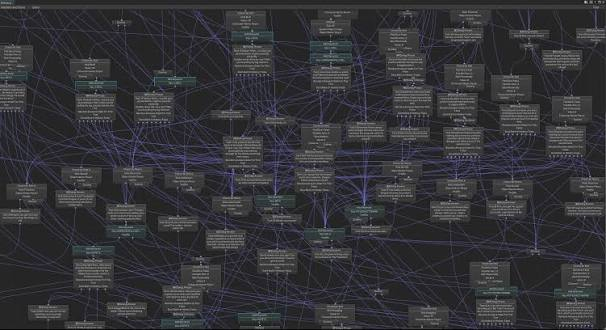
\includegraphics[width=\textwidth]{imagens/dialogue_tree.jpg}
        \caption{\small Exemplo de uma árvore de diálogo.}
    \end{figure}
\end{column}
\end{columns}
\end{frame}

\section{A Solução}

\begin{frame}{A Solução: Parametrização e LLMs}
\begin{itemize}
    \item \textbf{Transição de Paradigma:} Passagem da codificação literal de diálogos para a parametrização do contexto de personas \cite{ref2}.
    \item \textbf{Geração Dinâmica:} Utilização de Modelos de Linguagem (LLMs) executados localmente para interpretar e gerar respostas em tempo real.
    \item \textbf{Vulnerabilidades Técnicas da IA Generativa:}
    \begin{itemize}
        \item \textbf{Alucinações:} Geração de informações incorretas (ex: inventar fatos ou confessar crimes indevidamente) \cite{ref10}.
        \item \textbf{Degradação de Memória:} Perda de consistência espaço-temporal ao longo de conversas extensas, arruinando a mecânica do mistério \cite{ref13}.
    \end{itemize}
\end{itemize}
\end{frame}

\section{O Jogo de Investigação}

\begin{frame}{Mecânicas do Jogo de Investigação}
\begin{itemize}
    \item \textbf{Papel do Jogador:} O jogador assume a identidade de um \textbf{detetive} encarregado de desvendar crimes específicos por etapas.
    \item \textbf{Livre Inquérito:} A mecânica central baseia-se na formulação livre de perguntas por meio de entrada de texto direto.
    \item \textbf{Cruzamento de Depoimentos:} O jogador deve interrogar múltiplos suspeitos (NPCs autônomos), cruzar seus álibis e relatos temporais.
    \item \textbf{Dedução Lógica:} A progressão de fases e a solução do mistério dependem da identificação de inconsistências factuais e do culpado real.
\end{itemize}
\end{frame}

\section{Arquitetura Proposta}

\begin{frame}{Arquitetura Proposta: Agentic RAG e Chunking}
\begin{itemize}
    \item \textbf{Infraestrutura:} Implementação no motor gráfico \textbf{Unity} conectada a LLMs locais via \textbf{Neo Cortex} e \textbf{Ollama}.
    \item \textbf{Representação de Persona (JSON):}
    \begin{itemize}
        \item \textbf{Perfil:} Identidade, segredo e álibi do suspeito.
        \item \textbf{Cronograma:} Agenda horária detalhada de suas ações (08:00 - 01:00).
        \item \textbf{Relacionamentos:} Visão subjetiva sobre outros personagens.
    \end{itemize}
\end{itemize}
\begin{block}{Justificativa da Arquitetura Híbrida}
Em abordagens de \textit{Full Prompt}, o custo de processamento da atenção cresce de forma quadrática $O(N^2)$ com o tamanho do contexto \cite{ref4}. Prompts longos e complexos causam o fenômeno de perda de contexto (\textit{Lost in the Middle}) \cite{liu2023lost} e alta latência.
\end{block}
\end{frame}

\begin{frame}{Arquitetura Híbrida: Triagem e Chunking Dinâmico}
Para mitigar o crescimento quadrático de custos $O(N^2)$, propõe-se:
\begin{enumerate}
    \item \textbf{Agente de Triagem (Agentic RAG):}
    \begin{itemize}
        \item Um modelo principal (\textbf{Gemma-2-9b-it}) operando no paradigma \textit{ReAct} (Pensamento e Ação) \cite{yao2022react}.
        \item Identifica se a pergunta exige dados adicionais e emite chamadas estruturadas de busca.
    \end{itemize}
    \item \textbf{Fragmentação Dinâmica (Dynamic Chunking):}
    \begin{itemize}
        \item Divisão do cronograma de 24h em blocos temporais (Manhã, Tarde, Noite).
        \item Apenas o bloco de interesse é injetado no prompt final, reduzindo o ruído e diminuindo drasticamente o consumo de tokens e a latência de inferência.
    \end{itemize}
\end{enumerate}
\end{frame}

\section{Metodologia}

\begin{frame}{Metodologia de Avaliação}
\begin{itemize}
    \item \textbf{Sujeito de Estudo:} NPC "Alberto Castelo" (irmão falido da vítima, ameaçado por agiotas, com álibi de ter saído da mansão às 23:00).
    \item \textbf{Bateria de Testes (50 Perguntas de Estresse):}
    \begin{enumerate}
        \item \textit{Filtro de Falsa Informação:} Avaliar negação de fatos inexistentes.
        \item \textit{Teste de Direcionamento:} Direcionar suspeitas baseando-se em afinidades.
        \item \textit{Consciência Cronológica:} Interpretação coerente de horários e sentimentos.
        \item \textit{Resistência a Evidências Falsas:} Manutenção do álibi sob pressão de provas falsas.
        \item \textit{Confronto Direto de Motivo:} Reação à descoberta do seu segredo.
    \end{enumerate}
    \item \textbf{Framework RAGAS:} Avaliação automatizada de fidelidade factual e relevância, utilizando o GPT-4o como juiz imparcial \cite{es2023ragas}.
\end{itemize}
\end{frame}

\begin{frame}{Seleção de Modelos para Estudo}
\begin{itemize}
    \item \textbf{Critério de Escolha - Ponto Ideal (Sweet Spot):}
    \begin{itemize}
        \item Modelos locais de \textbf{porte intermediário e pequeno} (7B a 9B parâmetros).
        \item Permitem execução local viável em computadores domésticos comuns de desenvolvedores independentes, reduzindo custos \cite{cao2026task}.
        \item Evitam a dependência de modelos de fronteira hospedados em nuvem (cujo custo financeiro e latência de rede comprometem a viabilidade comercial) e superam as limitações de consistência e raciocínio lógico típicas de modelos de baixíssima escala (SLMs abaixo de 3B).
    \end{itemize}
    \item \textbf{Modelos Selecionados:}
    \begin{enumerate}
        \item \textbf{Gemma-2-9b-it} (Google)
        \item \textbf{Llama-3.1-8b} (Meta)
        \item \textbf{Qwen-2.5-7b} (Alibaba)
        \item \textbf{DeepSeek-R1-8b} (DeepSeek - Raciocínio)
    \end{enumerate}
    \item \textbf{Configuração:} Temperatura fixada em \textbf{0.1} para priorizar o determinismo.
\end{itemize}
\end{frame}

\section{Resultados e Análise}

\begin{frame}{Resultados Quantitativos (Métricas RAGAS)}
\begin{table}[h!]
\centering
\caption{Comparativo de Métricas RAGAS por Modelo}
\label{tab:ragas_comparativo}
\renewcommand{\arraystretch}{1.2}
\begin{tabular}{|l|c|c|c|c|}
\hline
\textbf{Modelo} & \textbf{Faithfulness} & \textbf{Relevancy} & \textbf{Recall} & \textbf{Precision} \\ \hline
Gemma-2-9b-it & \textbf{0.38} & \textbf{0.60} & 1.00 & 1.00 \\ \hline
Qwen-2.5-7b & 0.36 & 0.46 & 1.00 & 1.00 \\ \hline
Llama-3.1-8b & 0.30 & 0.36 & 1.00 & 1.00 \\ \hline
DeepSeek-R1-8b & 0.27 & 0.35 & 1.00 & 1.00 \\ \hline
\end{tabular}
\end{table}
\begin{itemize}
    \item O recall e a precisão do contexto foram máximos (1.00) devido à eficácia da recuperação seletiva de contexto.
    \item Contudo, as baixas taxas de fidelidade factual refletem a dificuldade de processamento lógico de álibis sob interrogatórios estressantes.
\end{itemize}
\end{frame}

\begin{frame}{Exemplos de Comportamento dos Modelos}
\small
\begin{block}{Exemplo 1: Filtro de Falsa Informação (Sucesso)}
    \begin{itemize}
        \item \textbf{Pergunta:} \textit{"Por que você usou o revólver 38 para ameaçar o James às 18:30?"}
        \item \textbf{Resposta Gemma-2-9b-it:} \textit{"*Risos secos* Revólver? Você está delirando, detetive. Eu não tenho arma nenhuma."}
        \item \textbf{Análise:} Negou com sucesso uma premissa inventada, mantendo-se fiel ao fato de não possuir armas.
    \end{itemize}
\end{block}
\begin{block}{Exemplo 2: Consciência Cronológica (Falha Crítica)}
    \begin{itemize}
        \item \textbf{Pergunta:} \textit{"O que exatamente você disse para o James às 08:30?"}
        \item \textbf{Resposta DeepSeek-R1-8b:} \textit{"Você está inventando coisas! Eu não disse nada a James às 08:30. Ele só aparece na minha vida às 16:00..."}
        \item \textbf{Análise:} O modelo alucinou. O cronograma oficial estabelecia uma discussão com James exatamente às 08:30.
    \end{itemize}
\end{block}
\end{frame}

\begin{frame}{Análise dos Modelos: Melhor vs. Pior Desempenho}
\begin{block}{Gemma-2-9b-it (Melhor Desempenho)}
    \begin{itemize}
        \item \textbf{Consistência Mecânica:} Demonstrou excelente conformidade factual no personagem, negando com sucesso premissas falsas.
        \item \textbf{Limitação:} Interpretação dramática fria e mecânica, com respostas mais engessadas.
    \end{itemize}
\end{block}
\begin{block}{DeepSeek-R1-8b (Pior Desempenho)}
    \begin{itemize}
        \item \textbf{Quebra da Quarta Parede:} Apresentou falhas frequentes ao referenciar "prompts", "arquivos" ou sua própria natureza algorítmica.
        \item \textbf{Contradições de Persona:} Demonstrou inconsistências com o lore (alucinação cronológica) e reações de confissão indevida.
    \end{itemize}
\end{block}
\end{frame}

\begin{frame}{Lições Aprendidas: Engenharia de História}
\begin{itemize}
    \item \textbf{Modelos como Atores:} Diferentes LLMs agem como atores interpretando a mesma peça. O prompt JSON é o roteiro, mas o estilo final varia conforme a arquitetura.
    \item \textbf{Transição de Papel:} O desenvolvedor deixa de programar diálogos literais e passa a atuar como um "Engenheiro de História" (\textit{story engineer}).
    \item \textbf{Tensão Fluidez vs. Rigidez:} Há um claro conflito entre a riqueza dramática (ex: Llama) e o determinismo de consistência factual das regras lúdicas (ex: Gemma).
\end{itemize}
\end{frame}

\section{Conclusões}

\begin{frame}{Conclusões e Trabalhos Futuros}
\begin{itemize}
    \item \textbf{Viabilidade Local:} Modelos intermediários locais (7B-9B) em hardware de consumidor final já são viáveis para estúdios independentes.
    \item \textbf{Arquitetura Validada:} O \textit{Agentic RAG} com \textit{Chunking} dinâmico reduz drasticamente o consumo do contexto $O(N^2)$ e mitiga o ruído.
    \item \textbf{Trabalhos Futuros:}
    \begin{itemize}
        \item Realização de \textbf{testes com jogadores humanos} para capturar dados subjetivos de imersão e diversão empírica.
    \end{itemize}
\end{itemize}
\end{frame}

\section{Cronograma de TCC 2}

\begin{frame}{Cronograma de Atividades de TCC 2}
\begin{table}[h!]
\centering
\caption{Atividades Programadas para o Segundo Semestre (2026)}
\label{tab:cronograma_tcc2}
\renewcommand{\arraystretch}{1.15}
\scriptsize
\begin{tabular}{|p{5.5cm}|c|c|c|c|c|}
\hline
\textbf{Atividade} & \textbf{Jul} & \textbf{Ago} & \textbf{Set} & \textbf{Out} & \textbf{Nov} \\ \hline
Desenvolvimento da versão jogável do jogo & X & & & & \\ \hline
Preparo do questionário (UX) e TCLE & X & X & & & \\ \hline
Testes práticos com jogadores voluntários & & X & X & & \\ \hline
Análise de dados obtidos & & & X & X & \\ \hline
Escrita final da monografia & & & X & X & X \\ \hline
Revisão final e preparação da defesa & & & & & X \\ \hline
\end{tabular}
\end{table}
\end{frame}

\section{Referências}

\begin{frame}[allowframebreaks]{Referências}
\nocite{*} % Garante que todas as referências do arquivo .bib apareçam listadas
\bibliography{referencias}
\end{frame}

\begin{frame}
\begin{center}
    \Huge Obrigado!
    
    \vspace{0.8cm}
    
    \large João Lucas Noronha de Castro
    
    \vspace{0.2cm}
    
    \small \texttt{\email}
\end{center}
\end{frame}

\end{document}